\documentclass[a4paper,12pt]{report}
\usepackage[utf8]{inputenc}
\usepackage[T1]{fontenc}
\usepackage{ngerman}

\usepackage{courier}
\usepackage{helvet}
\renewcommand{\rmdefault}{phv} 

\usepackage{geometry}
\geometry{a4paper,left=2cm,right=2cm, top=2cm, bottom=3cm}

\usepackage{graphicx} 

\usepackage{listings}
\lstdefinelanguage{drools}{
  morekeywords={rule,end,when,then},
  morecomment=[l]{//}, morecomment=[s]{/*}{*/},
}
\lstdefinelanguage{droolsfacts}{
  morekeywords={Input,OC,MC,Num,Solution},
  morecomment=[l]{//}, morecomment=[s]{/*}{*/},
}

\usepackage[plainpages=false,pdftitle={Business Rules in Semantic Wikis},pdfauthor={Sebastian Furth, Alexander Legler, Florian Ziegler}]{hyperref}

\begin{document}
  \pagenumbering{alph}
  
  \begin{titlepage}    
    \begin{center}
      \large{Julius-Maximilians-Universität Würzburg}
      
      \vspace{5cm}
      
      \huge{Softwarepraktikum}\\[1cm]
      \huge{\textbf{Business Rules in Semantic Wikis}}\\[2cm]
      
      \LARGE{
        Sebastian Furth\\[.25cm]
        Alexander Legler\\[.25cm]
        Florian Ziegler\\[.25cm]
      }
      
      \vspace{3cm}
      4. März 2010
    \end{center}
  \end{titlepage}
  
  \pagenumbering{arabic}
  
  \tableofcontents
  
  \parindent 0pt
  \parskip 9pt
  
  \chapter{Business Rules}

Eine \textbf{Business Rule} ist ein Ausdruck, der zur Problemlösung innerhalb eines Prozesses oder
einer abgegrenzten Aufgabenstellung beitragen kann. Business Rules können sowohl in Form von 
Beschreibungen als auch von Einschränkungen auftreten. 

Es gibt eine Vielzahl von Business Rule Management Systemen (BRMS). Zu den Bekanntesten gehören
JESS sowie das im Rahmen dieser Arbeit betrachtete JBoss Drools.

In diesem Bericht wird die Integration von JBoss Drools in ein bestehendes Wissensmanagementsystem
in Form eines Semantic Web Wikis beschrieben.

  \chapter{Kollaboratives Knowledge Engineering in Wikis}
  
  \section{Klassisches und kollaboratives KE}

Das Knowledge Engineering sollte insbesondere in seiner klassischen und der kollaborativen Form
unterschieden werden. 

Das klassiche Knowledge Engineering baut vorallem auf das Expertenwissen einer begrenzten
Anzahl von Personen (Community of Practice) und den methodischen Fähigkeiten eines 
Wissensingenieurs hinsichtlich Formalisierungsaspekten. 

Beim kollaborativen Knowledge Engineering steht der Gedanke des verteilten Wissens im Vordergrund.
Hierbei sollte besonders an Web-Communities gedacht werden, welche einen großen Wissensbestand, 
allerdings keine geeignete Plattform zu deren gezielter Verwaltung besitzen.


  \section{Möglichkeiten zum kollaborativen KE}

Zur Wissensaquise in kollaborativen Umgebungen eignen sich unterschiedlichste Methoden, wie z.B.
Web-Portale, Foren und Wikis. Wie am Beispiel der freien Enzyklopädie Wikipedia zu erkennen ist,
eignen sich Wikis hervorragend zur Sammlung von Wissen. Da dieses Wissen allerdings nur informell
vorliegt, bedarf es einer Möglichkeit zur Formalisierung. Diese Lücke wird durch das Semantic Web Wiki
KnowWE geschlossen.
  
  \section{Was ist KnowWE?}

KnowWE (Knowledge Wiki Environment) ist "`[e]in Semantisches Wiki, welches auf dem open-source Wiki JSPWiki 
aufbaut. Problemlösungswissen kann direkt im Wiki editiert und ausgeführt werden. Die im Wiki entwickelten 
Wissensbasen können exportiert und beispielsweise in OEM oder embedded Anwendungen verwendet werden. Weiterhin 
kann das Wissen über die Ontologiesprache OWL ausgetauscht werden."'\footnote{Nach: Seite „D3web“. In: Wikipedia, Die freie Enzyklopädie.}

\begin{figure}[htbp]
  \centering
    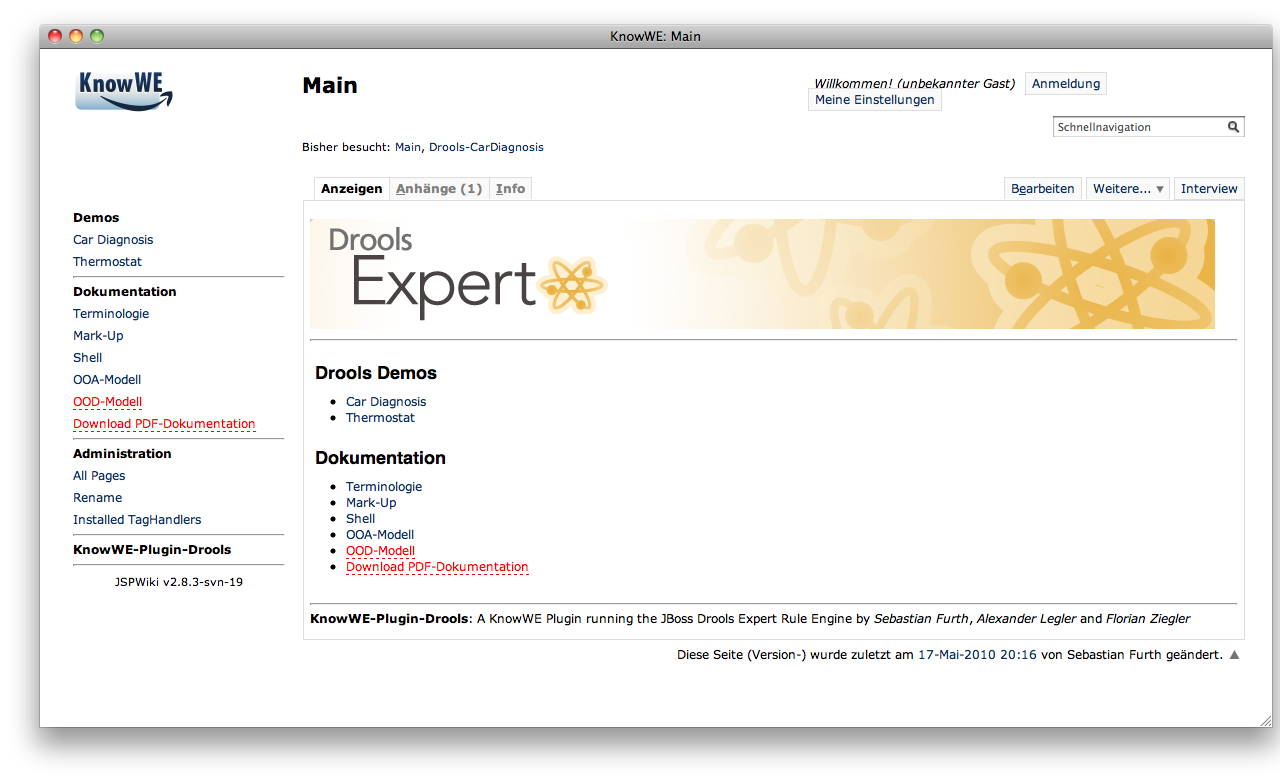
\includegraphics[width=\textwidth]{img/knowwe.png}
  \caption{Screenshot des Interfaces von KnowWE}
\end{figure}

  \chapter{Technische Umsetzung}

  \section{Technische Grundlagen von KnowWE}
    % jsps, servlets
    % knowweobjecttypes, taghandler, actions
    %   ^ ^ ^ ^ ^ 
    % kdom section

KnowWE basiert auf drei Grundkonzepten: \textbf{ObjectTypes}, \textbf{Taghandler} und \textbf{Actions}.

ObjectTypes übernehmen die Kernaufgabe der Wissensformalisierung. Daneben werden Taghandler insbesondere 
zum Rendering von Benutzerinteraktionselementen verwendet. Auf das Konzept der Actions wird zurückgegriffen 
wenn Benutzereingaben verarbeitet werden sollen.

  \section{Terminologie im DroolsPlugin}
  
  \begin{figure}[htbp]
    \centering
      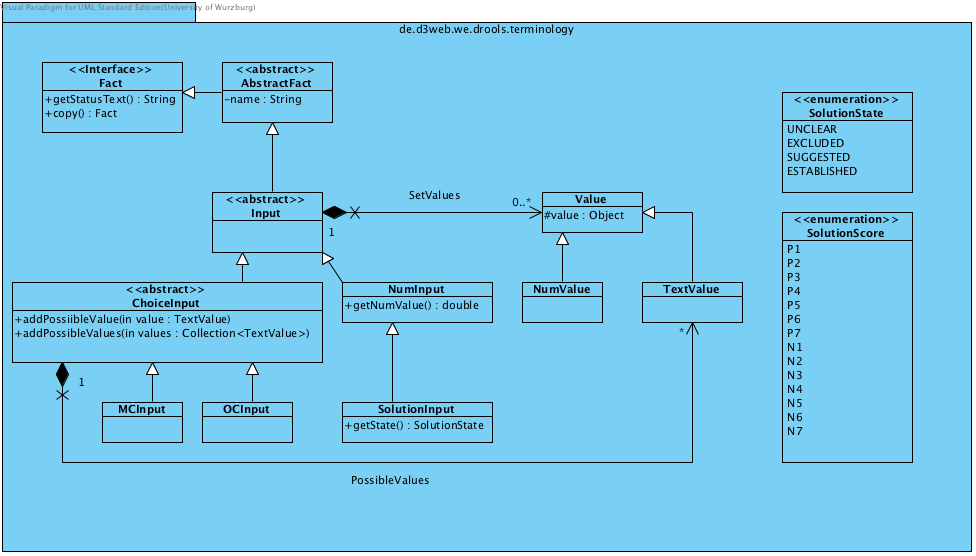
\includegraphics[width=\textwidth]{img/Terminologie.png}
    \caption{UML-Klassendiagramm des Pakets \texttt{d3.d3web.we.drools.terminology}}
    \label{fig:uml_terminology}
  \end{figure}
  
Die Terminologie im DroolsPlugin fußt auf zwei Kernkonzepten: \textbf{Inputs} und \textbf{Values}, wie in Abbildung \ref{fig:uml_terminology} gezeigt.

Inputs kapseln zumeist die im System vorhandenen Fragen und bieten je nach Ausprägung verschiedene Möglichkeiten für die Beantwortung an.

Values sind Objektcontainer, die zum Setzen von Werten in Inputs verwendet werden. 

  \subsection{Inputs}

Bei den Inputs sind \texttt{ChoiceInput}, \texttt{NumInput} sowie \texttt{SolutionInput} zu unterscheiden.

  \subsubsection{ChoiceInput}
Ein \texttt{ChoiceInput} lässt sich nach der Anzahl von Antwortmöglichkeiten in \texttt{MultipleChoiceInput}
und \texttt{OneChoiceInput} klassifizieren. Die Anzahl der Antwortmöglichkeiten definiert
wieviele Values gleichzeitig in einem \texttt{ChoiceInput} gesetzt sein dürfen. Die Antwortmöglichkeiten
sind außerdem durch die \texttt{PossibleValues} eingegrenzt, welche eine dem \texttt{ChoiceInput} fest zugeordnete 
Menge von Values darstellt.

  \subsubsection{NumInput} % (fold)

Ein \texttt{NumInput} kann nur einen einzigen numerischen Wert in Form eines \texttt{NumValue} aufnehmen.
  
  \subsubsection{SolutionInput}
Ein \texttt{SolutionInput} stellt eine besondere Form von \texttt{NumInput} dar und ist um eine \texttt{getState()}-Methode ergänzt, 
welche eine textuelle Repräsentation des momentanen numerischen Werts in Form eines \texttt{SolutionState} zurückgibt. 
Der numerische Wert der \texttt{SolutionInput} ist das Ergebnis des heuristischen Problemlösungsmechanismus, der 
mithilfe der Drools-Regeln integriert wurde.

Der Problemlösungsmechanismus beruht dabei auf den Werten der folgenden Tabelle:

\begin{table}[!h]
\begin{tabular}{r|c|c|c|c|c|c|c||c|c|c|c|c|c|c}

\textbf{Score} & N7 & N6 & N5 & N4 & N3 & N2 & N1 & P1 & P2 & P3 & P4 & P5 & P6 & P7\\
\hline
\textbf{Wert} & -999 & -80 & -40 & -20 & -10 & -5 & -2 & 2 & 5 & 10 & 20 & 40 & 80 & 999\\
\hline
\textbf{State} & \multicolumn{5}{c|}{\textbf{EXCLUDED}} & \multicolumn{4}{c|}{\textbf{UNCLEAR}} & \multicolumn{3}{c|}{\textbf{SUGGESTED}} & \multicolumn{2}{c}{\textbf{ESTABLISHED}}
\end{tabular}
\caption{Übersicht über vorgegebene Scores}
\end{table}

Abhängig von der Regel werden dem Score Punkte hinzugefügt oder abgezogen. Der State ergibt sich aus der momentanen Gesamtpunktzahl. Initial ist der Score eines
SolutionInputs 0.

  \subsection{Values}

Das DroolsPlugin definiert die \texttt{NumValue} und \texttt{TextValue}-Typen.
Ein \texttt{TextValue} nimmt einen beliebigen String-Inhalt auf und kann einem \texttt{ChoiceInput} zugeordnet werden,
Der \texttt{NumValue} hat zwei Funktionen: Er kapselt einen double-Wert zum einen für die Verwendung 
mit einem \texttt{NumInput} und zugleich stellt er die Scoring-Grundlage für die 
heuristische Problemlösung im \texttt{SolutionInput} dar.
  
  \section{Wiki-Markup}
  
Für das Markup werden drei Sections definiert, die \textbf{DroolsFactsSection}, welche die Terminologie beinhaltet, 
die \textbf{DroolsRulesSection}, welche das Regelwissen bereitstellt sowie die \textbf{DroolsSessionSection}, welche 
Befehle speichern und nacheinander abarbeiten kann.
  
  \subsection{DroolsFactsSection}
  
  Die Terminologie wird in der DroolsFactsSection durch typisierte \texttt{Input}-Statements definiert.
  Gültige Input-Typen sind \texttt{OC}, \texttt{MC}, \texttt{Num} und \texttt{Solution}, die im Folgenden erklärt werden.
  Sämtliche Objekte werden dem \emph{working memory} von Drools zugeführt.
  
  \lstset{numbers=left, numberstyle=\tiny, basicstyle=\small\ttfamily, stepnumber=1, numbersep=5pt, language=droolsfacts, breaklines=true, breakatwhitespace=true}
  \begin{lstlisting}[caption=Beispiel DroolsFactsSection]
  %%DroolsFacts
  Input<OC>("Starter", {"does not turn over", "turns over"});
  Input<MC>("Driving", {"insufficient power on partial load", "insufficient power on full load", "unsteady idle speed", "no /else"});
  Input<Num>("Year of construction");
  Input<Solution>("Bad ignition timing");
  Input<Solution>("Flat battery");
  %    
  \end{lstlisting}
  
  \subsubsection{One Choice Inputs}
  
  Der One Choice Input stellt eine Einfachauswahlmöglichkeit bereit. Hier wird ein OC-Input \texttt{Starter} definiert, welcher zwei mögliche Antwortalternativen bietet: \texttt{does not turn over} und \texttt{turns over}.
  
  \begin{lstlisting}
  Input<OC>("Starter", {"does not turn over", "turns over"});
  \end{lstlisting}
  
  \subsubsection{Multiple Choice Inputs}
  Der Multiple Choice Input erlaubt es, mehrere Antwortalternativen auszuwählen. Im Beispiel ist \texttt{Driving} ein MC-Input mit folgenden Antwortmöglichkeiten:
  \texttt{insufficient power on partial load}, \texttt{insufficient power on full load}, \texttt{unsteady idle speed} sowie \texttt{no /else}.
  
  \begin{lstlisting}
  Input<MC>("Driving", {"insufficient power on partial load", "insufficient power on full load", "unsteady idle speed", "no /else"});
  \end{lstlisting}

  \subsubsection{Numerical Inputs}
  
  Bei \texttt{Year of Construction} handelt es sich um einen numerischen Input, der keine Vorgabewerte hat.
  \begin{lstlisting}
  Input<Num>("Year of construction");
  \end{lstlisting}
  
  \subsubsection{Solution Inputs}
  \texttt{Bad ignition timing} und \texttt{Flat battery} stellen Lösungs-Inputs dar, d.h. sie stellen Lösungen wiederum in Input-Form dar, um eine Abstraktionsmöglichkeit
  innerhalb des Systems zu gewährleisten.
  
  \begin{lstlisting}  
  Input<Solution>("Bad ignition timing");
  Input<Solution>("Flat battery");
  \end{lstlisting}
  
  \subsection{DroolsRulesSection}
  
  In der DroolsRulesSection wird das Regelwissen formalisiert. Hierbei wird das Format der DRL, der Drools Rule Language verwendet. 
  
  \lstset{numbers=left, numberstyle=\tiny, basicstyle=\small\ttfamily, stepnumber=1, numbersep=5pt, language=drools, breaklines=true}  
  \begin{lstlisting}[caption=Beispiel DroolsRulesSection]
  %%DroolsRules
  rule "Flat battery"
    when
      $value : Value(value == "does not turn over")
      Input(name == "Starter" && values contains $value)
      $solution : SolutionInput(name == "Flat battery")
    then
      $solution.setValue(P5);
  end
  
  rule "Exclusion of bad ignition timing"
    when
      $value : Value(value == "turns over")
      not Input(name == "Starter" && values contains $value)
      $solution : SolutionInput(name == "Bad ignition timing")
    then
      $solution.setValue(N7);
  end
  
  %
  \end{lstlisting}
  
  Jede Regel besteht aus einem Titel ("`Flat battery"'), einem Bedingungsteil (\texttt{when}…), sowie einem Aktionsteil (\texttt{then}…).
  
  Grundsätzlich ist bei der Formulierung der Regeln zu beachten, dass die Fact-Bezeichner \emph{case-sensitive} sind.
  
  Im Bedingungsteil werden die Vorbedingungen formuliert, welche erfüllt sein müssen, damit diese Regel feuern kann.
  Ferner werden Variablen initialisiert, welche im Aktionsteil benötigt werden.
  
  In der Beispielregel "`Flat battery"' wird zunächst der Value \texttt{does not turn over} aus dem working memory von Drools abgerufen und
  überprüft, ob der Input mit der Bezeichnung \texttt{Starter} auf diesen Value gesetzt ist. Anschließend wird die Variable \texttt{\$solution} 
  initialisiert, welche für den Aktionsteil benötigt wird.
  
  Im Aktionsteil wir der zuvor initialisierten \texttt{\$solution}-Variable der Wert \texttt{P5} hinzugefügt.
  
  \subsection{DroolsSessionSection}

Zum schnelleren Zugriff auf Input/Value-Kombinationen bietet das Drools Plugin die Möglichkeit, sogenannte \textbf{Sessions} zu laden und zu speichern.
Mittels der Kommandos \texttt{store} und \texttt{load}, die weiter unten beschrieben werden, können Sessions gespeichert und
geladen werden.

Das Drools Plugin serialisiert die Session im folgenden Format:

\begin{lstlisting}[caption=Beispiel DroolsSessionSection]
%%DroolsSession
get Starter
set Starter = does not turn over
fire
get Flat battery

@Name:Foo
%
\end{lstlisting}

Beim Laden der Session werden die gespeicherten Befehle von oben nach unten abgearbeitet. Anzumerken ist, dass Sessions
auch manuell im Wiki-Artikel angelegt werden können.

  \section{Die Drools Shell}

Die Drools Shell ist das zentrale Interaktionselemnt des DroolsPlugins. Über sie werden sämtliche Eingaben und Ausgaben getätigt.
  
  \begin{figure}[htbp]
    \centering
      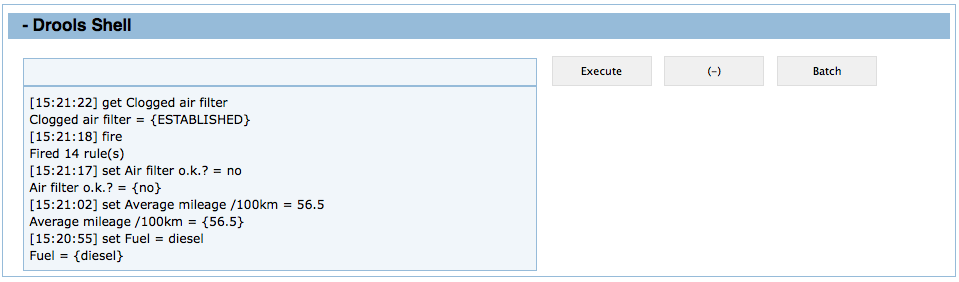
\includegraphics[width=\textwidth]{img/shell.png}
    \caption{Screenshot der Drools Shell mit Benutzersession}
    \label{fig:screen_shell}
  \end{figure}


  \begin{figure}[htbp]
    \centering
      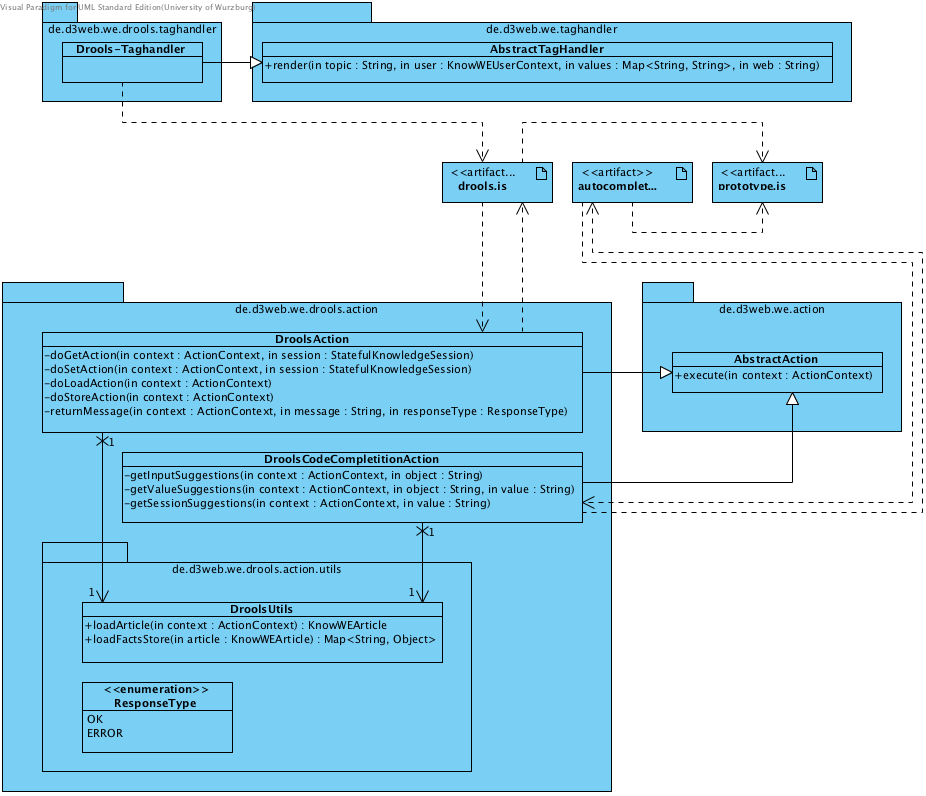
\includegraphics[width=\textwidth]{img/Actionkram.png}
    \caption{UML-Klassendiagramm der Drools Shell-Implementierung}
    \label{fig:uml_shell}
  \end{figure}

Der technische Aufbau wird anhand des UML-Diagramms in Abbildung \ref{fig:uml_shell} erklärt.

  Ausgangspunkt bildet der \texttt{DroolsTagHandler} welcher ein HTML-Formular mit Textfeld sowie drei Buttons "`Execute"', "`-/+"' und "`Batch"' in die Wiki-Seite rendert. Das Formular kann über den "`Execute"'-Button oder alternativ per Tastendruck auf <Enter> abgeschickt werden. Der "`-/+"'-Button blendet die History der Shell aus bzw. wieder ein. Ein Klick auf den "`Batch"'-Button führt dazu, dass sich die Eingabezeile in ein Eingabefeld verwandelt, in welches mehrere Befehle zeilenweise eingegeben werden können. Zu beachten ist hierbei, dass sich das Formular nicht mehr mit <Enter> abschicken lässt, sondern <Shift> + <Enter> gedrückt werden müssen. 
  
  Die vom Benutzer eingegebenen Daten werden zunächst von den hinterlegten JavaScript-Funktionen entgegengenommen und anschließend per AJAX\footnote{Asynchronous JavaScript and XML} an die \texttt{DroolsAction} und \texttt{DroolsCodeCompletionAction} gesendet und dort verarbeitet. Die DroolsAction übernimmt dabei die Interaktion mit der Terminologie und den hinterlegetne Regeln. Auf die Funktionsweise der DroolsCodeCompletionAction wird in einem separaten Punkt genauer eingegangen.

  Das Ergebnis der Verarbeitung wird KnowWE-typisch über die \texttt{KnowWE.jsp} an den Client ausgegeben. Von dort werden sie dann wieder per Javascript verarbeitet und auf der Konsole ausgegeben. 


  \subsection{Benutzung}
  \subsubsection{Verfügbare Kommandos}
  
  \begin{tabular}{l|p{320pt}}

  \textbf{Komanndo} & \textbf{Erklärung}\\
  \hline
  
  \texttt{help} & Gibt alle verfügbaren Befehle auf der Drools Shell aus.\\
  \texttt{get <Input>} & Gibt den aktuellen Wert (Value) eines Inputs aus.\\
  \texttt{set <Input> = <Value>} & Setzt den Wert eines Inputs auf den übergebenen Value.\\
  \texttt{fire} & Feuert alle passenden Regeln.\\
  \texttt{reset} & Setzt alle Inputs auf ihre Ausgangswerte zurück.\\
  \texttt{clear} & Leert die Konsole.\\
  \texttt{store <Name>} & Speichert alle zuvor eingegebene Befehle unter dem eingegebenen Namen als DroolsSession.\\
  \texttt{load <Name>} & Lädt die zuvor gespeicherte DroolsSession <Name> in die aktuelle Sitzung.\\
  
  \end{tabular}
  
    % store und load besonders beschreiben...

  \subsubsection{Autocompletion}
  
  Zur einfachen Bedienung der Drools-Shell wird der Benutzer durch die DroolsCodeCompletionAction bei seinen Eingaben unterstützt. Dies geschieht im wesentlichen dadurch, dass zu seinen bisherigen Eingaben Vorschläge unterhalb der Konsole eingeblendet werden. 
  
  \begin{figure}[htbp]
    \centering
      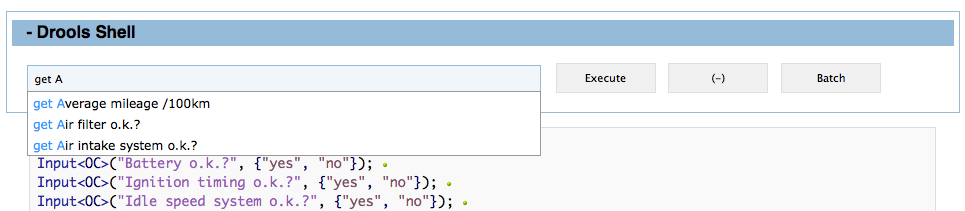
\includegraphics[width=\textwidth]{img/shell-autocomplete.png}
    \caption{Screenshot der Drools Shell mit Autocompletion-Feature}
  \end{figure}
  
  Wie dem obigen Beispiel zu entnehmen ist, wird die Benutzereingabe "`get a"' durch drei Vorschläge unterstützt. 
  Die Navigation innerhalb der Vorschläge erfolgt über die Pfeiltasten.

  \appendix
  
  \chapter{Gesamte UML-Diagramme}
  \section{OOA-Model}
  
  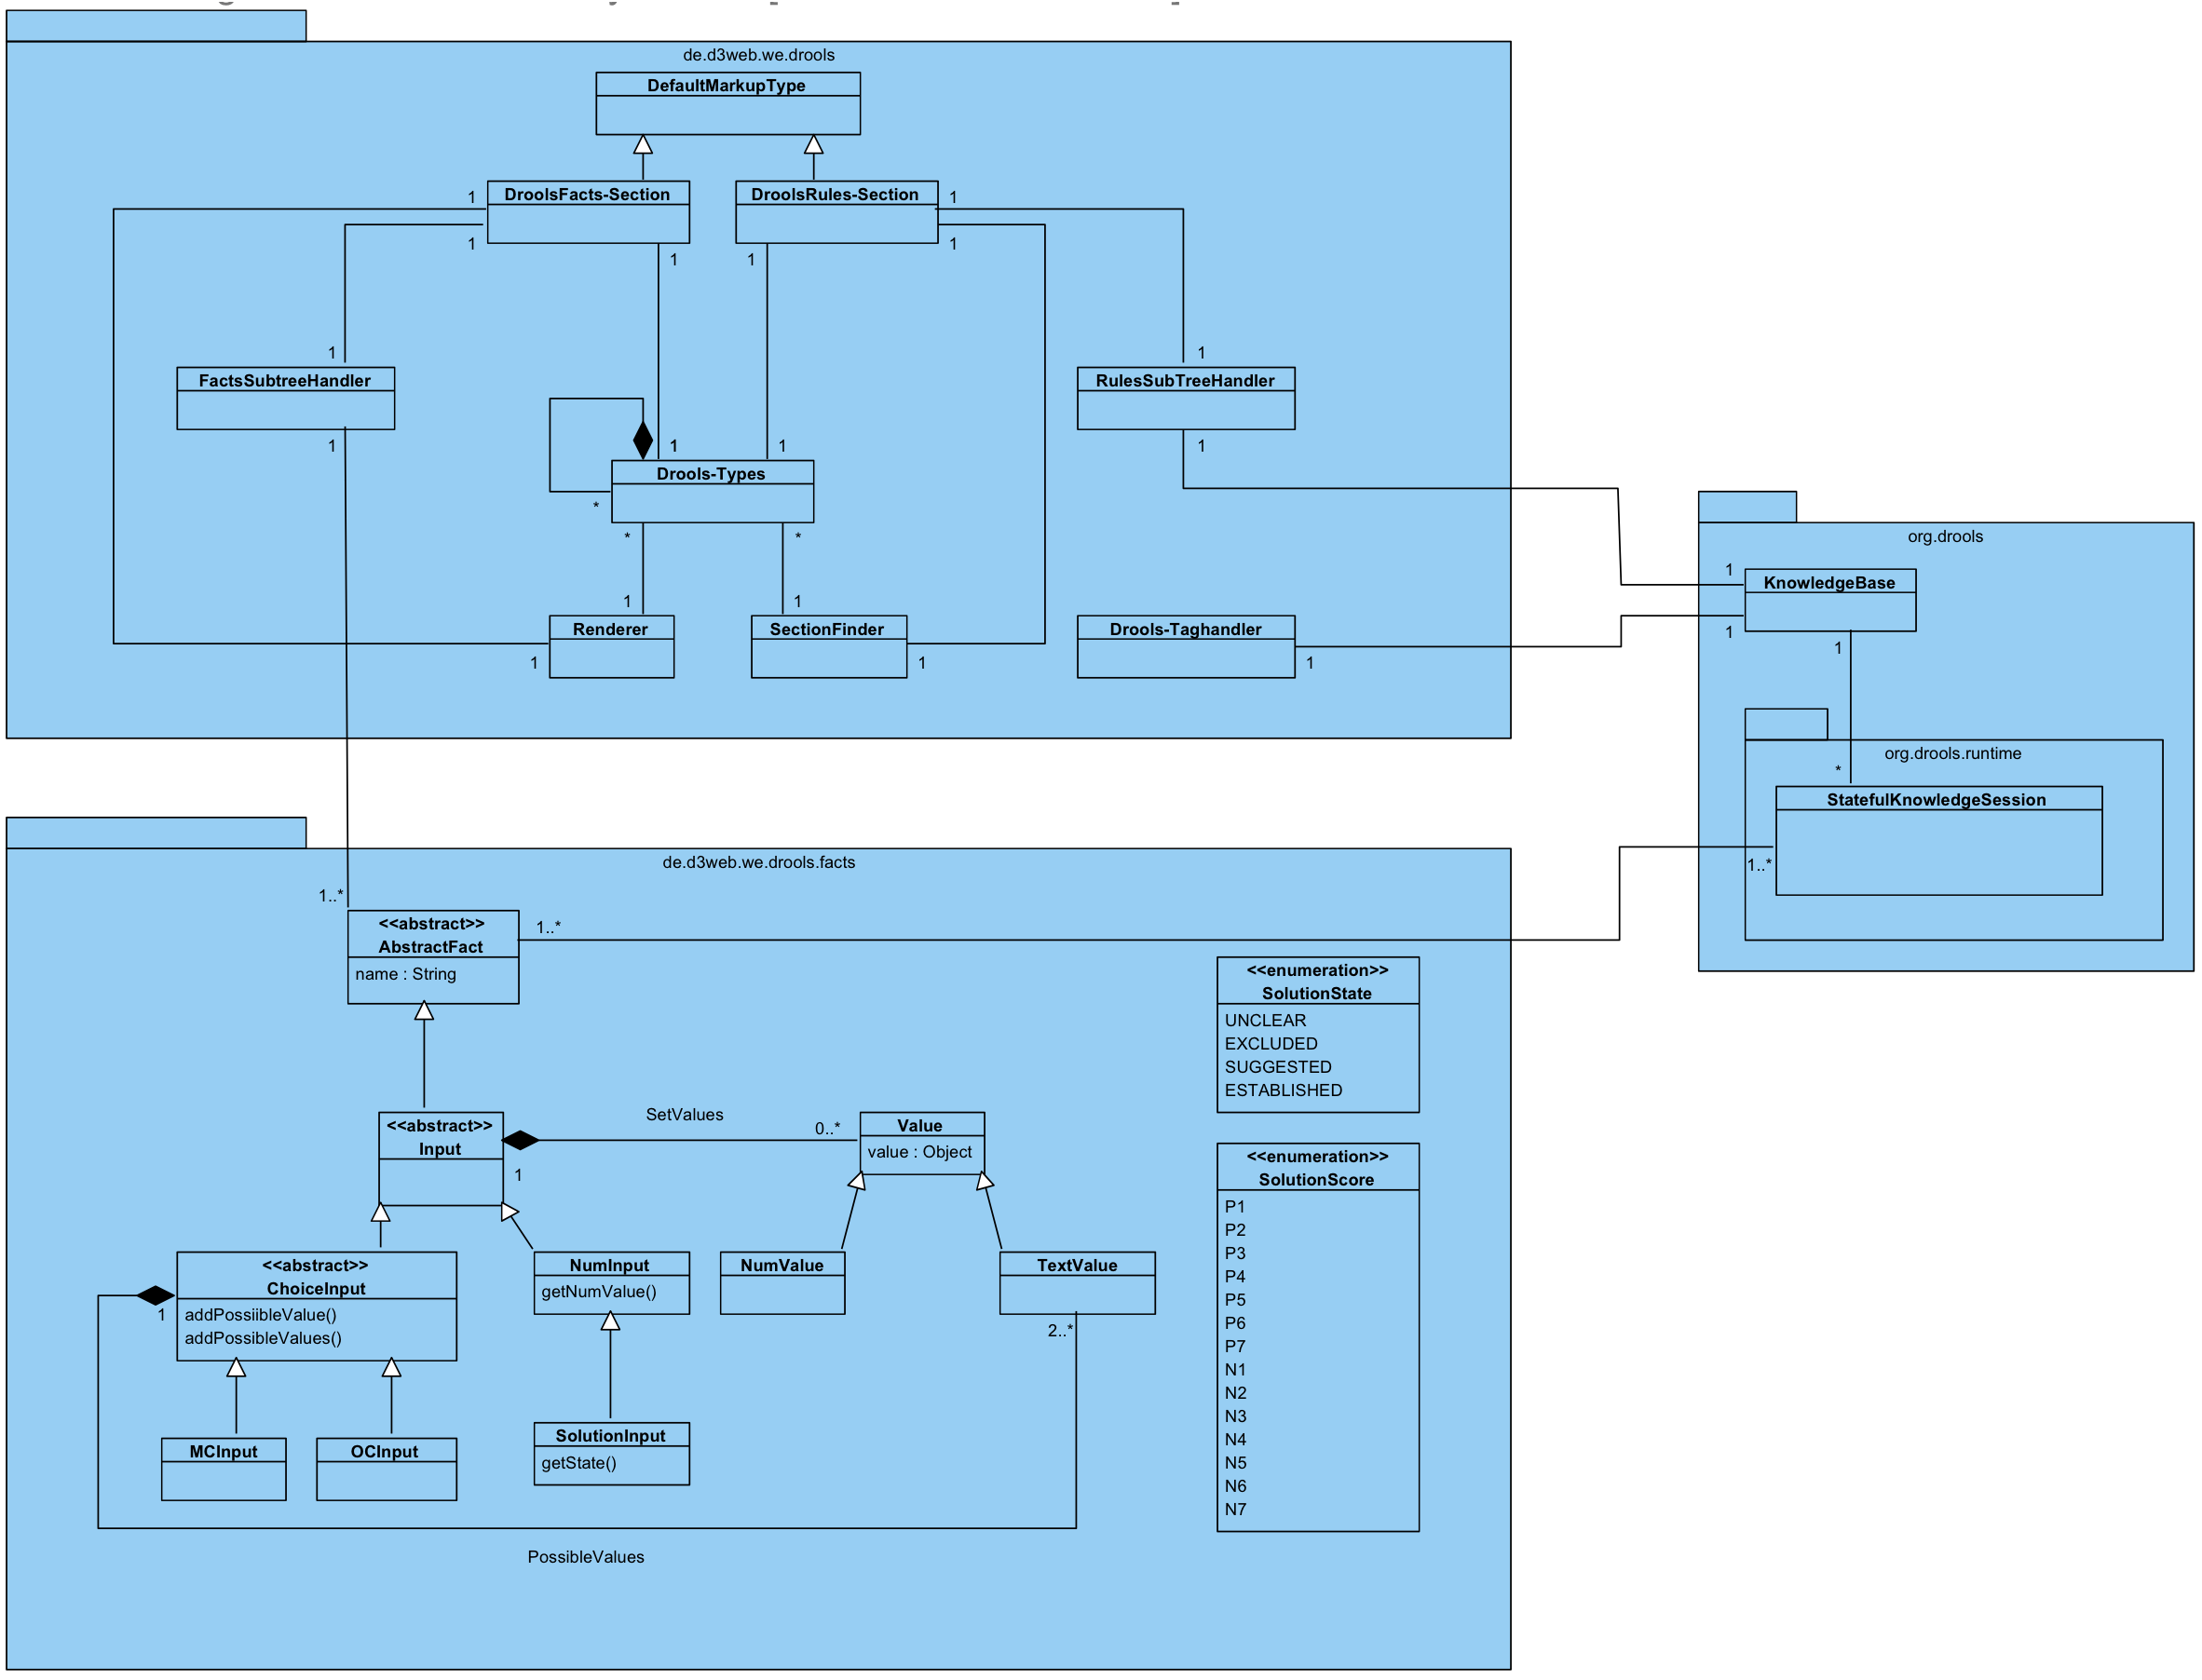
\includegraphics[width=\textwidth]{img/ooa.png}

  \section{OOD-Model}  
  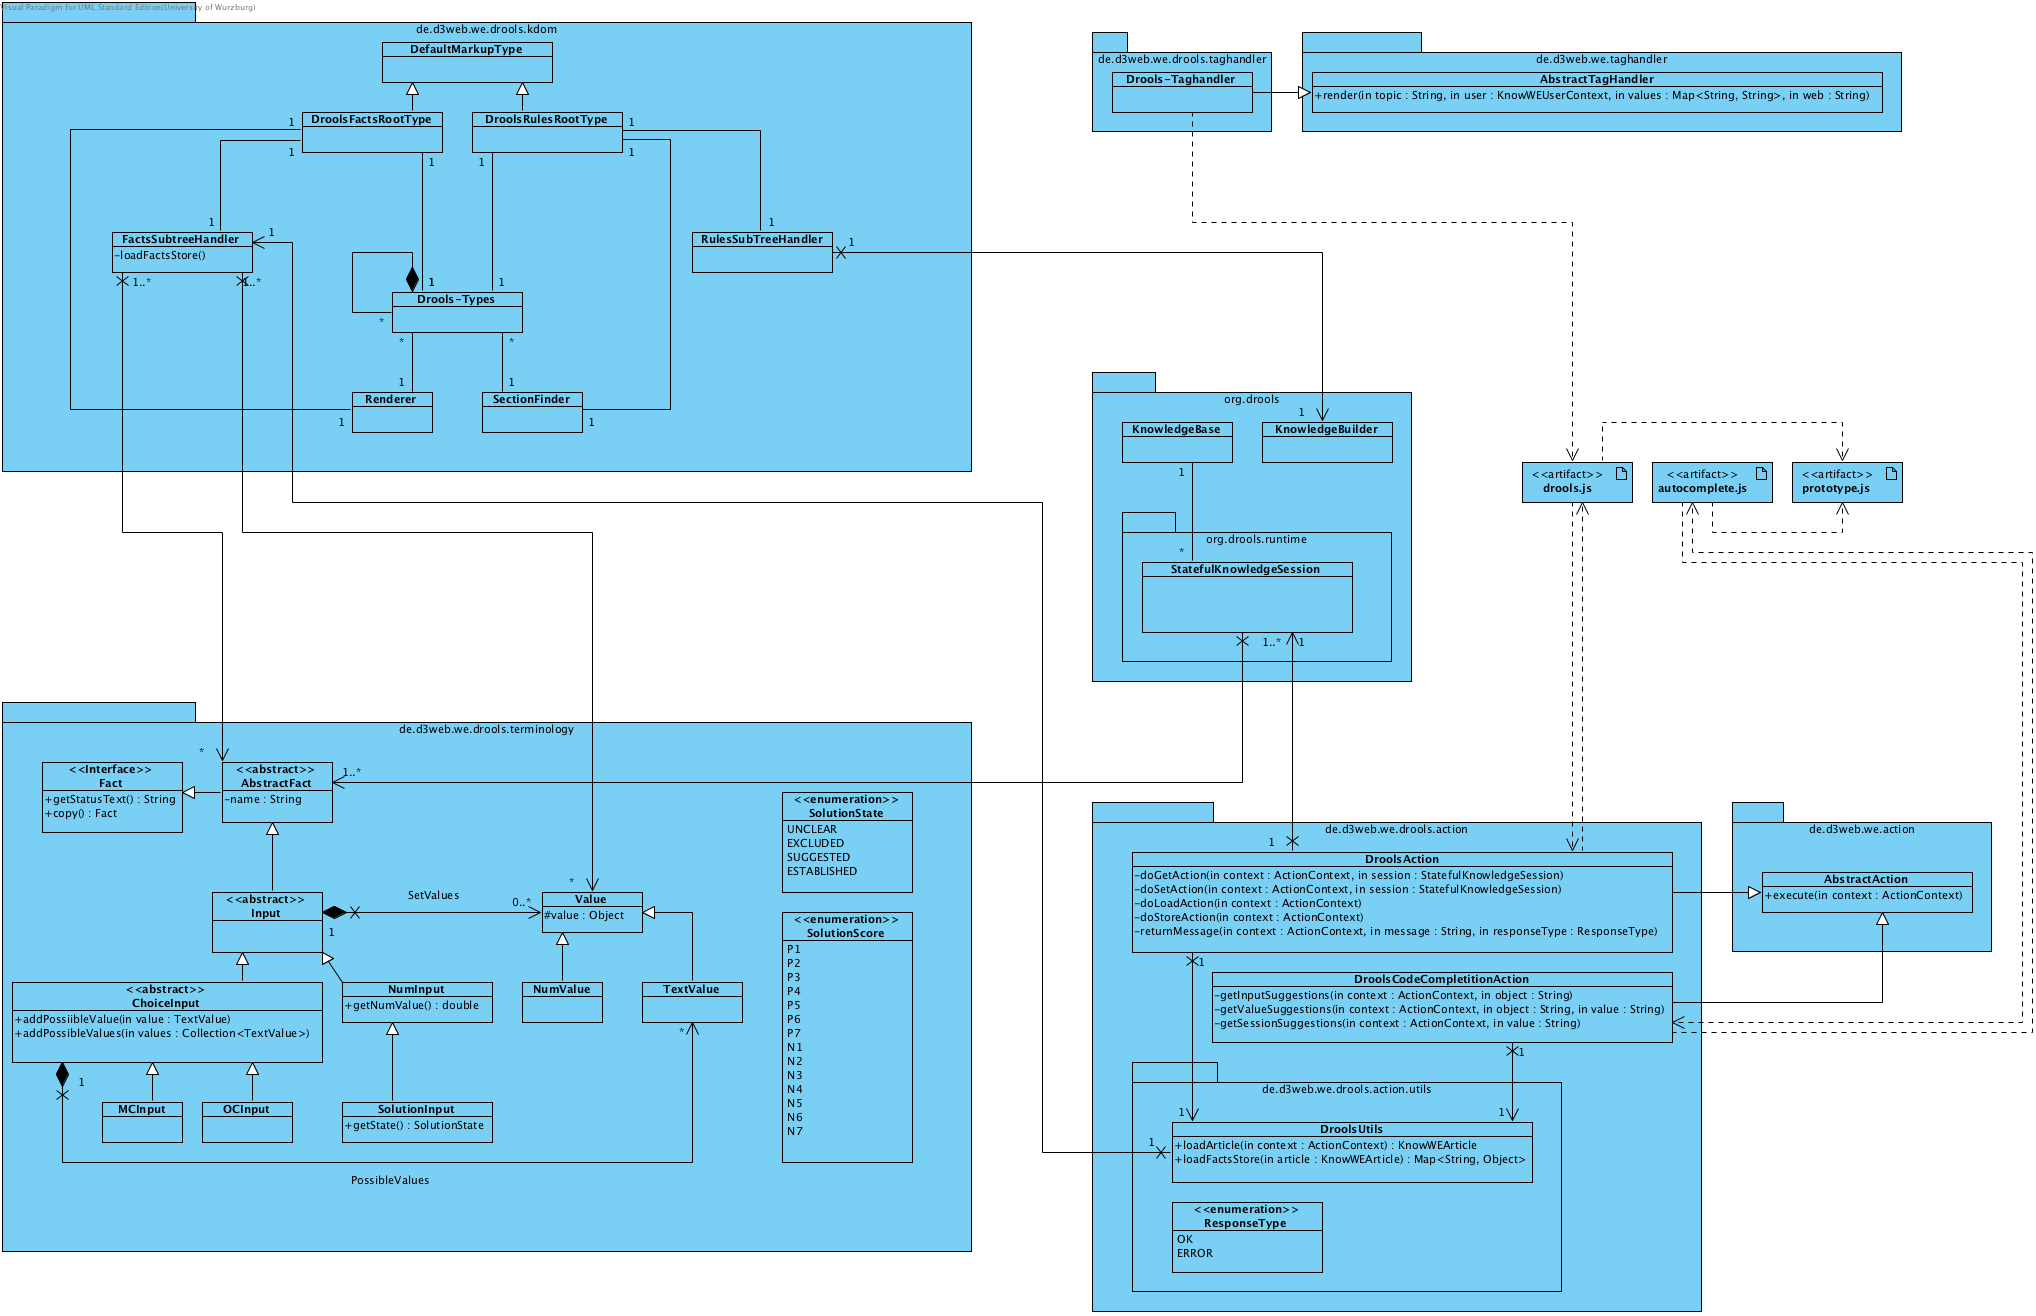
\includegraphics[height=15cm,angle=90]{img/ood.png}
  

  \chapter{Beispiel: Car Diagnosis}
  \begin{lstlisting}[]
  !!! Drools Demo - Car Diagnosis

  [{KnowWEPlugin drools}]

  %%DroolsFacts
  Input<OC>("Battery o.k.?", {"yes", "no"});
  Input<OC>("Ignition timing o.k.?", {"yes", "no"});
  Input<OC>("Idle speed system o.k.?", {"yes", "no"});
  Input<Num>("Year of construction");
  Input<OC>("Air filter o.k.?", {"yes", "no"});
  Input<OC>("Air intake system o.k.?", {"yes", "no"});
  Input<OC>("Starter", {"does not turn over", "turns over"});
  Input<OC>("Engine start", {"engine barely starts", "engine starts", "does not start"});
  Input<OC>("Make of car", {"VW", "Opel", "Mercedes Benz", "BMW", "Porsche", "Fiat", "Toyota", "Mazda", "Other"});
  Input<MC>("Driving", {"insufficient power on partial load", "insufficient power on full load", "unsteady idle speed", "low idle speed", "delayed take-off", "weak acceleration", "no /else"});
  Input<Num>("Average mileage /100km");
  Input<Num>("Num. Mileage evaluation");
  Input<OC>("Mileage evaluation", {"slightly increased", "normal", "increased"});
  Input<Num>("Real mileage  /100km");
  Input<OC>("Exhaust fumes", {"black", "blue", "invisible"});
  Input<OC>("Exhaust pipe color", {"brown", "grey", "light grey", "sooty black"});
  Input<OC>("Exhaust pipe color evaluation", {"abnormal", "normal"});
  Input<OC>("Fuel", {"diesel", "unleaded gasoline"});
  Input<OC>("Engine noises", {"knocking", "ringing", "no /else"});
  Input<Solution>("Damaged idle speed system");
  Input<Solution>("Leaking air intake system");
  Input<Solution>("Clogged air filter");
  Input<Solution>("Bad ignition timing");
  Input<Solution>("Empty battery");

  %

  %%DroolsRules
  rule "R7"
    when
      // This rule was converted manually
      $real : Input(name == "Real mileage  /100km" && numValue != 0)
      $average : Input(name == "Average mileage /100km" && numValue > 0.0)
      $input : NumInput(name == "Num. Mileage evaluation")
    then
      $input.setValue($real.getNumValue() / $average.getNumValue() * 100);
  end

  rule "R51"
    when
      $value : Value(value == "no")
      Input(name == "Battery o.k.?" && values contains $value)
      $solution : SolutionInput(name == "Empty battery")
    then
      $solution.setValue(P7);
  end

  rule "R52"
    when
      $value : Value(value == "yes")
      Input(name == "Battery o.k.?" && values contains $value)
      $solution : SolutionInput(name == "Empty battery")
    then
      $solution.setValue(N7);
  end

  rule "R53"
    when
      $value : Value(value == "does not turn over")
      Input(name == "Starter" && values contains $value)
      $solution : SolutionInput(name == "Empty battery")
    then
      $solution.setValue(P5);
  end

  rule "R54"
    when
      $value : Value(value == "turns over")
      Input(name == "Starter" && values contains $value)
      $solution : SolutionInput(name == "Empty battery")
    then
      $solution.setValue(N4);
  end

  rule "R55_1_2"
    when
      $value1 : Value(value == "engine barely starts")
      Input(name == "Engine start" && values contains $value1)
      $solution : SolutionInput(name == "Empty battery")
    then
      $solution.setValue(P5);
  end

  rule "R55_2_2"
    when
      $value2 : Value(value == "does not start")
      Input(name == "Engine start" && values contains $value2)
      $solution : SolutionInput(name == "Empty battery")
    then
      $solution.setValue(P5);
  end

  rule "R56"
    when
      $value : Value(value == "engine starts")
      Input(name == "Engine start" && values contains $value)
      $solution : SolutionInput(name == "Empty battery")
    then
      $solution.setValue(N5);
  end

  rule "R23"
    when
      $value : Value(value == "yes")
      Input(name == "Air intake system o.k.?" && values contains $value)
      $solution : SolutionInput(name == "Leaking air intake system")
    then
      $solution.setValue(N7);
  end

  rule "R24"
    when
      $value : Value(value == "no")
      Input(name == "Air intake system o.k.?" && values contains $value)
      $solution : SolutionInput(name == "Leaking air intake system")
    then
      $solution.setValue(P7);
  end

  rule "R16"
    when
      $value1 : Value(value == "insufficient power on full load")
      Input(name == "Driving" && values.size > 0  && values not contains $value1)
      $value3 : Value(value == "unsteady idle speed")
      Input(name == "Driving" && values.size > 0 && values not contains $value3)
      $value4 : Value(value == "insufficient power on partial load")
      Input(name == "Driving" && values.size > 0 && values not contains $value4)
      $solution : SolutionInput(name == "Leaking air intake system")
    then
      $solution.setValue(N3);
  end

  rule "R17"
    when
      $value : Value(value == "insufficient power on full load")
      Input(name == "Driving" && values contains $value)
      $solution : SolutionInput(name == "Leaking air intake system")
    then
      $solution.setValue(P5);
  end

  rule "R18"
    when
      $value : Value(value == "insufficient power on partial load")
      Input(name == "Driving" && values contains $value)
      $solution : SolutionInput(name == "Leaking air intake system")
    then
      $solution.setValue(P3);
  end

  rule "R19"
    when
      $value : Value(value == "unsteady idle speed")
      Input(name == "Driving" && values contains $value)
      $solution : SolutionInput(name == "Leaking air intake system")
    then
      $solution.setValue(P1);
  end

  rule "R20"
    when
      $value : Value(value == "slightly increased")
      Input(name == "Mileage evaluation" && values contains $value)
      $solution : SolutionInput(name == "Leaking air intake system")
    then
      $solution.setValue(P3);
  end

  rule "R21"
    when
      $value : Value(value == "normal")
      Input(name == "Mileage evaluation" && values contains $value)
      $solution : SolutionInput(name == "Leaking air intake system")
    then
      $solution.setValue(N4);
  end

  rule "R22"
    when
      $value : Value(value == "increased")
      Input(name == "Mileage evaluation" && values contains $value)
      $solution : SolutionInput(name == "Leaking air intake system")
    then
      $solution.setValue(P4);
  end

  rule "R10"
    when
      $value : Value(value == "engine barely starts")
      Input(name == "Engine start" && values.size > 0 && values not contains $value)
      $solution : SolutionInput(name == "Damaged idle speed system")
    then
      $solution.setValue(N5);
  end

  rule "R11"
    when
      $value : Value(value == "engine barely starts")
      Input(name == "Engine start" && values contains $value)
      $solution : SolutionInput(name == "Damaged idle speed system")
    then
      $solution.setValue(P5);
  end

  rule "R12"
    when
      $value : Value(value == "unsteady idle speed")
      Input(name == "Driving" && values.size > 0 && values not contains $value)
      $solution : SolutionInput(name == "Damaged idle speed system")
    then
      $solution.setValue(N1);
  end

  rule "R13"
    when
      $value : Value(value == "unsteady idle speed")
      Input(name == "Driving" && values contains $value)
      $solution : SolutionInput(name == "Damaged idle speed system")
    then
      $solution.setValue(P1);
  end

  rule "R14"
    when
      $value : Value(value == "low idle speed")
      Input(name == "Driving" && values.size > 0 && values not contains $value)
      $solution : SolutionInput(name == "Damaged idle speed system")
    then
      $solution.setValue(N4);
  end

  rule "R15"
    when
      $value : Value(value == "low idle speed")
      Input(name == "Driving" && values contains $value)
      $solution : SolutionInput(name == "Damaged idle speed system")
    then
      $solution.setValue(P4);
  end

  rule "R8"
    when
      $value : Value(value == "yes")
      Input(name == "Idle speed system o.k.?" && values contains $value)
      $solution : SolutionInput(name == "Damaged idle speed system")
    then
      $solution.setValue(N7);
  end

  rule "R9"
    when
      $value : Value(value == "no")
      Input(name == "Idle speed system o.k.?" && values contains $value)
      $solution : SolutionInput(name == "Damaged idle speed system")
    then
      $solution.setValue(P7);
  end

  rule "R31"
    when
      $value : Value(value == "abnormal")
      Input(name == "Exhaust pipe color evaluation" && values contains $value)
      $solution : SolutionInput(name == "Clogged air filter")
    then
      $solution.setValue(P5);
  end

  rule "R32"
    when
      $value : Value(value == "normal")
      Input(name == "Exhaust pipe color evaluation" && values contains $value)
      $solution : SolutionInput(name == "Clogged air filter")
    then
      $solution.setValue(N5);
  end

  rule "R38"
    when
      $value1 : Value(value == "engine barely starts")
      Input(name == "Engine start" && values.size > 0 && values not contains $value1)
      $value2 : Value(value == "does not start")
      Input(name == "Engine start" && values.size > 0 && values not contains $value2)
      $solution : SolutionInput(name == "Clogged air filter")
    then
      $solution.setValue(N4);
  end

  rule "R39_3_2"
    when
      $value3 : Value(value == "engine barely starts")
      Input(name == "Engine start" && values contains $value3)
      $solution : SolutionInput(name == "Clogged air filter")
    then
      $solution.setValue(P4);
  end

  rule "R39_4_2"
    when
      $value4 : Value(value == "does not start")
      Input(name == "Engine start" && values contains $value4)
      $solution : SolutionInput(name == "Clogged air filter")
    then
      $solution.setValue(P4);
  end

  rule "R40"
    when
      $value1 : Value(value == "engine barely starts")
      Input(name == "Engine start" && values.size > 0 && values not contains $value1)
      $value2 : Value(value == "does not start")
      Input(name == "Engine start" && values.size > 0 && values not contains $value2)
      $solution : SolutionInput(name == "Bad ignition timing")
    then
      $solution.setValue(N5);
  end

  rule "R41_3_2"
    when
      $value3 : Value(value == "engine barely starts")
      Input(name == "Engine start" && values contains $value3)
      $solution : SolutionInput(name == "Bad ignition timing")
    then
      $solution.setValue(P5);
  end

  rule "R41_4_2"
    when
      $value4 : Value(value == "does not start")
      Input(name == "Engine start" && values contains $value4)
      $solution : SolutionInput(name == "Bad ignition timing")
    then
      $solution.setValue(P5);
  end

  rule "R33"
    when
      $value1 : Value(value == "unleaded gasoline")
      Input(name == "Fuel" && values contains $value1)
      $value2 : Value(value == "black")
      Input(name == "Exhaust fumes" && values contains $value2)
      $solution : SolutionInput(name == "Clogged air filter")
    then
      $solution.setValue(P5);
  end

  rule "R25"
    when
      $value : Value(value == "yes")
      Input(name == "Air filter o.k.?" && values contains $value)
      $solution : SolutionInput(name == "Clogged air filter")
    then
      $solution.setValue(N7);
  end

  rule "R26"
    when
      $value : Value(value == "no")
      Input(name == "Air filter o.k.?" && values contains $value)
      $solution : SolutionInput(name == "Clogged air filter")
    then
      $solution.setValue(P7);
  end

  rule "R27"
    when
      $value1 : Value(value == "weak acceleration")
      Input(name == "Driving" && values.size > 0 && values not contains $value1)
      $value2 : Value(value == "unsteady idle speed")
      Input(name == "Driving" && values.size > 0 && values not contains $value2)
      $solution : SolutionInput(name == "Clogged air filter")
    then
      $solution.setValue(N5);
  end

  rule "R28"
    when
      $value : Value(value == "unsteady idle speed")
      Input(name == "Driving" && values contains $value)
      $solution : SolutionInput(name == "Clogged air filter")
    then
      $solution.setValue(P4);
  end

  rule "R29"
    when
      $value : Value(value == "weak acceleration")
      Input(name == "Driving" && values contains $value)
      $solution : SolutionInput(name == "Clogged air filter")
    then
      $solution.setValue(P5);
  end

  rule "R30"
    when
      $value : Value(value == "turns over")
      Input(name == "Starter" && values.size > 0 && values not contains $value)
      $solution : SolutionInput(name == "Clogged air filter")
    then
      $solution.setValue(N6);
  end

  rule "R34"
    when
      $value : Value(value == "black")
      Input(name == "Exhaust fumes" && values.size > 0 && values not contains $value)
      $solution : SolutionInput(name == "Clogged air filter")
    then
      $solution.setValue(N5);
  end

  rule "R35"
    when
      $value : Value(value == "slightly increased")
      Input(name == "Mileage evaluation" && values contains $value)
      $solution : SolutionInput(name == "Clogged air filter")
    then
      $solution.setValue(P3);
  end

  rule "R36"
    when
      $value : Value(value == "normal")
      Input(name == "Mileage evaluation" && values contains $value)
      $solution : SolutionInput(name == "Clogged air filter")
    then
      $solution.setValue(N4);
  end

  rule "R37"
    when
      $value : Value(value == "increased")
      Input(name == "Mileage evaluation" && values contains $value)
      $solution : SolutionInput(name == "Clogged air filter")
    then
      $solution.setValue(P4);
  end

  rule "R47"
    when
      $value : Value(value == "yes")
      Input(name == "Ignition timing o.k.?" && values contains $value)
      $solution : SolutionInput(name == "Bad ignition timing")
    then
      $solution.setValue(N7);
  end

  rule "R48"
    when
      $value : Value(value == "no")
      Input(name == "Ignition timing o.k.?" && values contains $value)
      $solution : SolutionInput(name == "Bad ignition timing")
    then
      $solution.setValue(P7);
  end

  rule "R46"
    when
      $value : Value(value == "turns over")
      Input(name == "Starter" && values.size > 0 && values not contains $value)
      $solution : SolutionInput(name == "Bad ignition timing")
    then
      $solution.setValue(N6);
  end

  rule "R49_1_2"
    when
      $value1 : Value(value == "knocking")
      Input(name == "Engine noises" && values contains $value1)
      $solution : SolutionInput(name == "Bad ignition timing")
    then
      $solution.setValue(P5);
  end

  rule "R49_2_2"
    when
      $value2 : Value(value == "ringing")
      Input(name == "Engine noises" && values contains $value2)
      $solution : SolutionInput(name == "Bad ignition timing")
    then
      $solution.setValue(P5);
  end

  rule "R50"
    when
      $value1 : Value(value == "knocking")
      Input(name == "Engine noises" && values.size > 0 && values not contains $value1)
      $value2 : Value(value == "ringing")
      Input(name == "Engine noises" && values.size > 0 && values not contains $value2)
      $solution : SolutionInput(name == "Bad ignition timing")
    then
      $solution.setValue(N3);
  end

  rule "R42"
    when
      $value1 : Value(value == "weak acceleration")
      Input(name == "Driving" && values.size > 0 && values not contains $value1)
      $value3 : Value(value == "unsteady idle speed")
      Input(name == "Driving" && values.size > 0 && values not contains $value3)
      $value4 : Value(value == "delayed take-off")
      Input(name == "Driving" && values.size > 0 && values not contains $value4)
      $solution : SolutionInput(name == "Bad ignition timing")
    then
      $solution.setValue(N4);
  end

  rule "R43"
    when
      $value : Value(value == "unsteady idle speed")
      Input(name == "Driving" && values contains $value)
      $solution : SolutionInput(name == "Bad ignition timing")
    then
      $solution.setValue(P1);
  end

  rule "R44"
    when
      $value : Value(value == "delayed take-off")
      Input(name == "Driving" && values contains $value)
      $solution : SolutionInput(name == "Bad ignition timing")
    then
      $solution.setValue(P3);
  end

  rule "R45"
    when
      $value : Value(value == "weak acceleration")
      Input(name == "Driving" && values contains $value)
      $solution : SolutionInput(name == "Bad ignition timing")
    then
      $solution.setValue(P4);
  end

  rule "R1"
    when
      $value1 : Value(value == "sooty black")
      Input(name == "Exhaust pipe color" && values contains $value1)
      $value2 : Value(value == "unleaded gasoline")
      Input(name == "Fuel" && values contains $value2)
      $input : ChoiceInput(name == "Exhaust pipe color evaluation")
    then
      $input.setValue("abnormal");
  end

  rule "R2"
    when
      $value1 : Value(value == "sooty black")
      Input(name == "Exhaust pipe color" && values contains $value1)
      $value2 : Value(value == "diesel")
      Input(name == "Fuel" && values contains $value2)
      $input : ChoiceInput(name == "Exhaust pipe color evaluation")
    then
      $input.setValue("normal");
  end

  rule "R4"
    when
      Input(name == "Num. Mileage evaluation" && numValue <= 130.0)
      Input(name == "Num. Mileage evaluation" && numValue >= 110.0)
      $input : ChoiceInput(name == "Mileage evaluation")
    then
      $input.setValue("slightly increased");
  end

  rule "R5"
    when
      Input(name == "Num. Mileage evaluation" && numValue > 130.0)
      $input : ChoiceInput(name == "Mileage evaluation")
    then
      $input.setValue("increased");
  end

  rule "R6"
    when
      Input(name == "Num. Mileage evaluation" && numValue > 0 && numValue < 110.0)
      $input : ChoiceInput(name == "Mileage evaluation")
    then
      $input.setValue("normal");
  end

  rule "R3_1_2"
    when
      $value1 : Value(value == "light grey")
      Input(name == "Exhaust pipe color" && values contains $value1)
      $input : ChoiceInput(name == "Exhaust pipe color evaluation")
    then
      $input.setValue("normal");
  end

  rule "R3_2_2_3_2"
    when
      $value3 : Value(value == "grey")
      Input(name == "Exhaust pipe color" && values contains $value3)
      $input : ChoiceInput(name == "Exhaust pipe color evaluation")
    then
      $input.setValue("normal");
  end

  rule "R3_2_2_4_2"
    when
      $value4 : Value(value == "brown")
      Input(name == "Exhaust pipe color" && values contains $value4)
      $input : ChoiceInput(name == "Exhaust pipe color evaluation")
    then
      $input.setValue("normal");
  end

  %
  %%DroolsSession
  get Clogged air filter
  set Exhaust fumes = black
  set Fuel = unleaded gasoline
  set Engine start = engine barely starts
  fire
  get Clogged air filter

  @Name: CloggedAirFilter_Suggested
  %
    
  \end{lstlisting}
  
\end{document}